\documentclass{article}
\usepackage{amsmath, amssymb, graphicx}
\usepackage{hyperref}
\usepackage{geometry}
\geometry{a4paper, margin=1in}

\title{Time-Varying Graphical Lasso: Summary and Application}
\author{Your Name}
\date{}

\begin{document}

\maketitle

\tableofcontents

\section{Article Summarization and Theoretical Formulation}
\label{sec:summary_theory}

\subsection{Introduction}
\label{subsec:intro}

In many applications, such as finance, neuroscience, and social networks, relationships between variables evolve over time. Modeling these dynamics is critical for understanding and predicting system behavior. The \textbf{Time-Varying Graphical Lasso (TVGL)} extends the classical Graphical Lasso to infer sparse precision matrices (inverse covariance matrices) that vary smoothly over time. This allows for the simultaneous discovery of network structures and their temporal evolution.

\vspace{0.5em}
\noindent\textbf{Motivation and Setting:}
\begin{itemize}
    \item Standard Graphical Lasso assumes data are independent and identically distributed (i.i.d.) and estimates a single sparse precision matrix $\Theta$.
    \item In time-dependent settings, relationships among variables evolve, requiring a framework that captures temporal variations while preserving sparsity.
    \item TVGL addresses this by introducing temporal penalties to encourage smooth transitions in precision matrices.
\end{itemize}

\vspace{0.5em}
\noindent\textbf{Applications:}
\begin{itemize}
    \item \textit{Finance}: Evolving correlations among stocks under changing market conditions.
    \item \textit{Neuroscience}: Brain connectivity changes with cognitive tasks or disease progression.
    \item \textit{Social Networks}: Shifting user interactions over time.
\end{itemize}

\subsection{Theoretical Importance of the Inverse Covariance Matrix}
\label{subsec:importance_inverse_cov}

The inverse covariance matrix, also known as the precision matrix, plays a crucial role in understanding the relationships among variables in multivariate data. It encodes the conditional independence structure of the variables:

\vspace{0.5em}
\noindent\textbf{Conditional Independence:}
If the $(i,j)$-th entry of the precision matrix $\Theta = \Sigma^{-1}$ is zero, i.e., $\Theta_{ij} = 0$, then the variables $X_i$ and $X_j$ are conditionally independent given all other variables in the system. Mathematically,
\begin{equation}
    \Theta_{ij} = 0 \quad \iff \quad P(X_i, X_j | X_{\backslash \{i,j\}}) = P(X_i | X_{\backslash \{i,j\}}) P(X_j | X_{\backslash \{i,j\}}).
\end{equation}
This makes the precision matrix a critical tool for understanding and visualizing dependencies in a network.

\vspace{0.5em}
\noindent\textbf{Proof:}
Given a multivariate Gaussian distribution $X \sim \mathcal{N}(\mu, \Sigma)$, the joint density is:
\begin{equation}
    f_X(x) = \frac{1}{(2\pi)^{p/2} |\Sigma|^{1/2}} \exp\left(-\frac{1}{2}(x - \mu)^T \Sigma^{-1} (x - \mu)\right).
\end{equation}
The conditional density of $X_i$ given $X_{\backslash i}$ can be derived from the joint Gaussian density. The conditional independence between $X_i$ and $X_j$ given $X_{\backslash \{i,j\}}$ follows directly from the structure of $\Sigma^{-1}$:
\begin{itemize}
    \item If $\Theta_{ij} = 0$, the $(i,j)$ entry in the inverse covariance matrix, this implies that there is no direct dependency between $X_i$ and $X_j$ when conditioned on the remaining variables.
    \item This property simplifies network interpretation by representing the dependencies through the graph encoded by $\Theta$.
\end{itemize}

\vspace{0.5em}
\noindent\textbf{Real-World Implications:}
In practice, this property of the precision matrix is used in:
\begin{itemize}
    \item \textit{Neuroscience:} Identifying functional connectivity in the brain by analyzing relationships between different regions over time.
    \item \textit{Finance:} Understanding dependencies between assets and mitigating risk by identifying conditional independencies.
    \item \textit{Genomics:} Mapping gene interactions by inferring sparse dependencies between genes.
\end{itemize}

\subsection{Theoretical Formulation}
\label{subsec:theory}

\subsubsection{Problem Definition and Objective}
Given a sequence of empirical covariance matrices $\{S_t\}_{t=1}^T$ computed from time-dependent data, the goal is to estimate precision matrices $\{\Theta_t\}_{t=1}^T$ for each time step $t$. The objective combines likelihood-based data fidelity, sparsity, and temporal smoothness:

\begin{equation}
\min_{\Theta_1, \ldots, \Theta_T \succ 0} \quad \sum_{t=1}^T \Big[-n_t \log \det(\Theta_t) + n_t \mathrm{Tr}(S_t \Theta_t) \Big] + \lambda \sum_{t=1}^T \|\Theta_t\|_{\text{offdiag},1} + \beta \sum_{t=2}^T \psi(\Theta_t - \Theta_{t-1}),
\end{equation}

where:
\begin{itemize}
    \item $-n_t \log \det(\Theta_t) + n_t \mathrm{Tr}(S_t \Theta_t)$: Negative log-likelihood for Gaussian data.
    \item $\|\Theta_t\|_{\text{offdiag},1}$: Encourages sparsity by penalizing off-diagonal elements.
    \item $\psi(\cdot)$: Temporal penalty encouraging smooth transitions between consecutive matrices.
    \item $\lambda, \beta$: Regularization parameters controlling sparsity and smoothness.
\end{itemize}

\subsubsection{Choices for Temporal Penalty $\psi$}
Different penalties model various evolutionary patterns:
\begin{itemize}
    \item \textbf{Element-wise L1}: $\psi(X) = \|X\|_1$ for sparse edge changes.
    \item \textbf{Group Lasso (L2)}: $\psi(X) = \sum_j \|X_{:,j}\|_2$, enforcing node-wise changes.
    \item \textbf{Laplacian}: $\psi(X) = \|X\|_F^2$, favoring smooth variations.
    \item \textbf{Infinity Norm}: $\psi(X) = \|X\|_{\infty}$ for block-wise changes.
    \item \textbf{Perturbed Node}: A row-column overlap norm allowing single-node rewiring.
\end{itemize}

\vspace{0.5em}
\noindent\textbf{Advantages of Temporal Penalties:}
\begin{itemize}
    \item \textbf{Sparsity}: Ensures the precision matrices are interpretable by promoting zero elements.
    \item \textbf{Smooth Transitions}: Captures gradual changes in relationships, reflecting real-world dynamics.
    \item \textbf{Flexibility}: Different penalties allow modeling various types of network evolution.
\end{itemize}

\subsection{Optimization Approach}
\label{subsec:optimization}

The TVGL optimization problem can be solved using:
\begin{itemize}
    \item \textbf{Interior-point methods}: Effective for small-scale problems.
    \item \textbf{First-order methods (e.g., ADMM)}: Scalable for large $p$ or $T$ by solving subproblems iteratively.
\end{itemize}

\vspace{0.5em}
\noindent\textbf{ADMM-based Approach:}
\begin{itemize}
    \item Splits the problem into smaller subproblems for each $\Theta_t$ and temporal penalty term.
    \item Ensures convergence to the global optimum with computational efficiency.
    \item Adapts well to high-dimensional settings by leveraging sparsity.
\end{itemize}

\vspace{0.5em}
\noindent\textbf{Challenges:}
\begin{itemize}
    \item High computational cost for large $T$ or $p$.
    \item Balancing sparsity and smoothness parameters ($\lambda$, $\beta$) requires careful tuning.
\end{itemize}



\section{Implementation Details and Testing on Synthetic Data}
\label{sec:implementation_synthetic}
\subsection{Implementation Details}
\label{subsec:Implementation Details}

\subsection{Synthetic Data Generation: Market Dynamics and Conditional Independence}
\label{subsec:synthetic_data}

\subsubsection{Objective}
The synthetic data aims to simulate market-like dynamics with two groups of stocks and their associated indices. The primary goal is to analyze conditional independence relationships, introduce a market event that shifts these dynamics, and test the ability of TVGL to estimate the evolving precision matrices.

\subsubsection{Setup and Dynamics}
\paragraph{Initial Configuration}
\begin{itemize}
    \item \textbf{Groups and Variables:}
    \begin{itemize}
        \item \textbf{Group 1:} 3 stocks and 1 index associated with these stocks.
        \item \textbf{Group 2:} 2 stocks and 1 index associated with these stocks.
    \end{itemize}

    \begin{figure}[h!]
    \centering
    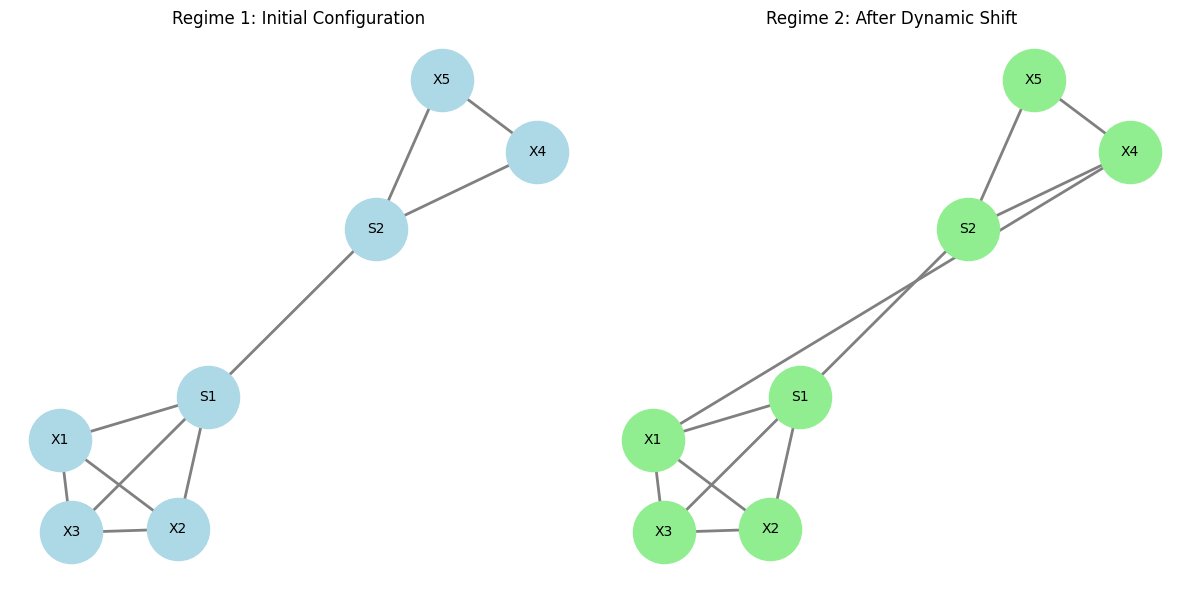
\includegraphics[width=\textwidth]{synthetic_data.png}
    \caption{Your caption here}
    \label{fig:label}
\end{figure}


    \item \textbf{Dynamic Relationships:}
    \begin{itemize}
        \item \textbf{Indexes:} Correlated and conditionally correlated. Knowing one index provides additional information about the other.
        \item \textbf{Stocks within a group:} Correlated and conditionally correlated. Knowing one stock provides information about others in the same group.
        \item \textbf{Stocks between groups:} Conditionally independent. Stocks in different groups are independent given the indices and other stocks in their respective groups.
    \end{itemize}
    \item \textbf{Matrix Constraints:}
    \begin{itemize}
        \item Precision matrix (inverse covariance matrix) reflects the dynamics, including zeros for conditional independence.
        \item Must be positive definite for invertibility.
    \end{itemize}
\end{itemize}

\paragraph{Market Change: Partial Acquisition Scenario}
\begin{itemize}
    \item \textbf{Dynamic Shift:} Partial acquisition between Group 1 and Group 2 changes the dynamics.
    \begin{itemize}
        \item Stocks in the two groups are no longer conditionally independent.
        \item Knowing a stock in one group provides additional information about stocks in the other group.
    \end{itemize}
    \item \textbf{Matrix Adjustment:}
    \begin{itemize}
        \item Update the precision matrix: Add non-zero coefficients for newly dependent variables.
        \item Ensure no changes to other zero coefficients to preserve the original conditional independence relationships.
        \item Maintain positive definiteness to ensure invertibility.
    \end{itemize}
\end{itemize}

\subsection{Implementation Plan}
\label{subsec:implementation_plan}

\paragraph{Step 1: Generate Initial Precision Matrix}
Construct the precision matrix to reflect the initial relationships:
\begin{itemize}
    \item Correlations between stocks and indexes within the same group.
    \item Conditional independence between groups.
\end{itemize}
Ensure positive definiteness of the precision matrix.

\paragraph{Step 2: Compute Covariance Matrix}
Compute the covariance matrix analytically as the inverse of the precision matrix.

\paragraph{Step 3: Generate Synthetic Data}
Use the covariance matrix to generate multivariate normal data for time horizon $T$.

\paragraph{Step 4: Modify Precision Matrix}
Adjust the precision matrix to reflect the new market dynamics:
\begin{itemize}
    \item Add non-zero coefficients for newly dependent variables.
    \item Preserve zero coefficients that correspond to conditional independence.
    \item Ensure the matrix remains positive definite and invertible.
\end{itemize}

\paragraph{Step 5: Generate Data for Updated Dynamics}
Compute the updated covariance matrix. Generate synthetic data for horizon $T'$.

\paragraph{Step 6: Concatenate Data and Estimate Relationships}
Concatenate data from the two horizons. Estimate the covariance matrices for both regimes using the synthetic data. Compute the precision matrices from the estimated covariance matrices.

\paragraph{Step 7: Analyze Results}
Identify pairs of variables that are conditionally independent in each regime. Compare the results to the theoretical precision matrices and highlight discrepancies where estimation produces incorrect results.

\subsection{Expected Insights}
\label{subsec:expected_insights}

\begin{itemize}
    \item \textbf{Initial Regime:} Clear identification of conditional independence based on the precision matrix.
    \item \textbf{Post-Acquisition Regime:} Correct reflection of new dependencies and preserved independencies.
    \item \textbf{Estimation Accuracy:} Precision matrix estimations may deviate from theoretical values, highlighting estimation limitations.
\end{itemize}




\end{document}
